\chapter{Design and Implementation}
In this chapter an in detail description is given for the software and hardware which has been implemented. Starting with \S~\ref{sec:imp-requirements} section which gives an overview of the most important requirements the software artefact should meet. \S~\ref{sec:imp-supportingTools} covers tools which have been developed in order to aid the use of the feedback system. Finlay the \S~\ref{sec:imp-systemArchitecture} section gives an indept description of the inner workings of the feedback system and how components integrate with each other. 

\section{Requirements}
\label{sec:imp-requirements}
The the feedback system is broken down into the following basic requirements.

\begin{description}
	\item[Abstract Input / Output Interface] The telemetry data input and feedback output needs to be abstracted. Techniclay this does not effect the feedback's effectiveness or accuracy but it is usefull as to be able to change the sim racing game and the type of feedback which is given with out having to change any of the internal components. This allows for fast prototyping especially with the output interface in which one can develop another way to convey the feedback. 
	\item[Perform Spatial Querying] The feedback system relies on being able to determine the location of the car on track. This is used to determine if the car is in a straight section or corner section, how far away from the race line the car is and if the mid point of the corner is being driven on. 
	\item[Store telemetry files] In order for the evaluation chapter to be carried out, the telemetry data is required to be stored for later data analysis. This is achieved by writing the telemetry data to a log file which is later uploaded to the database.
	\item[Query log files]
\end{description}

\subsection{Sim Racing Rig}
\label{sec:imp-simRacingRig}
The rig is made out of various independent components. The steering wheel is a Logitech G25 a pedal set, an H shifter and a bucket racing seat, all mounted on to a home made metal frame.

\begin{figure}[!htb]
	\centering
	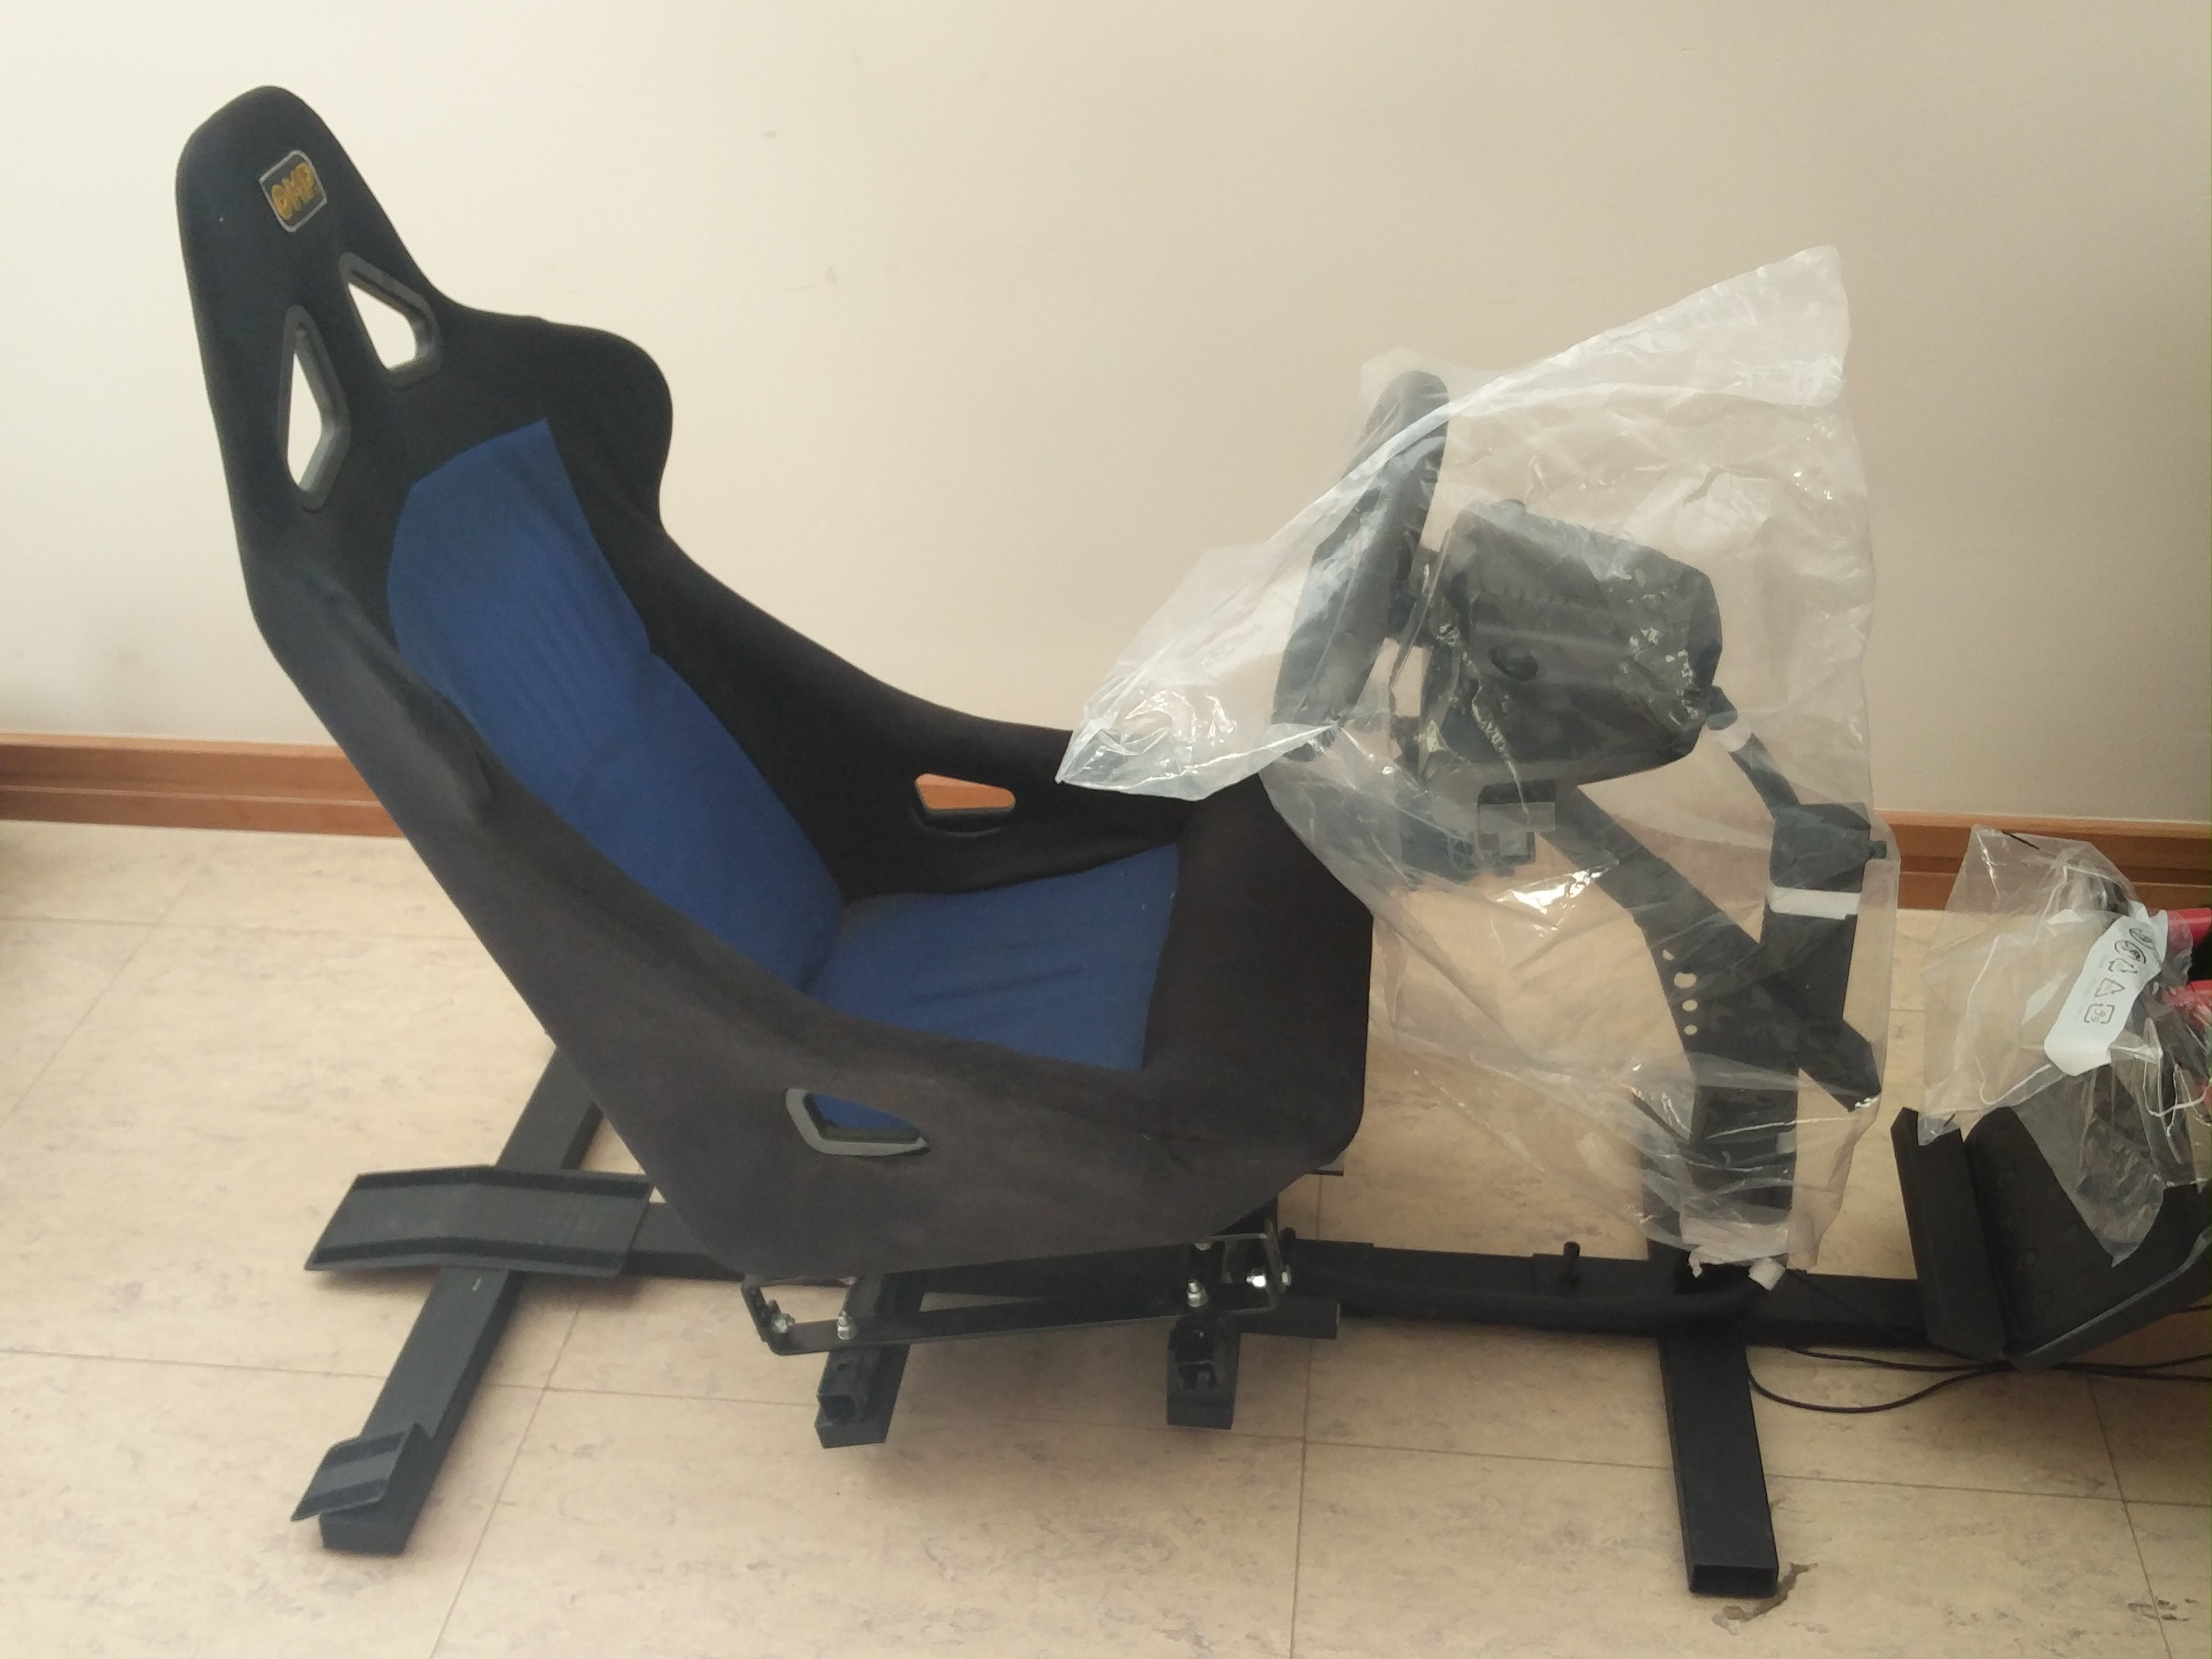
\includegraphics[height=5cm]{images/RacingRig}
	\caption{Side view of the racing rig}
	\label{fig:RacingRig}
\end{figure}

\section{Supporting tools}
\label{sec:imp-supportingTools}
In order to aid the feedback system, special tools have been developed in order to generate file which are required to make the feedback system work with a specific track

\subsection{Track Splicer}
\label{sec:imp-trackSplicer}
The track splicer tool has been developed to aid the feedback system's track meta data file creation. It automates the following tasks. Given a series of two dimensional cartesian coordinate denoting a track race line, (i) split the race line into straights and corners (ii) find the mid point of a corner which is used as the apex point and (iii) give a visual representation of the race line, straights and corners. 

\begin{figure}[!htb]
	\centering
	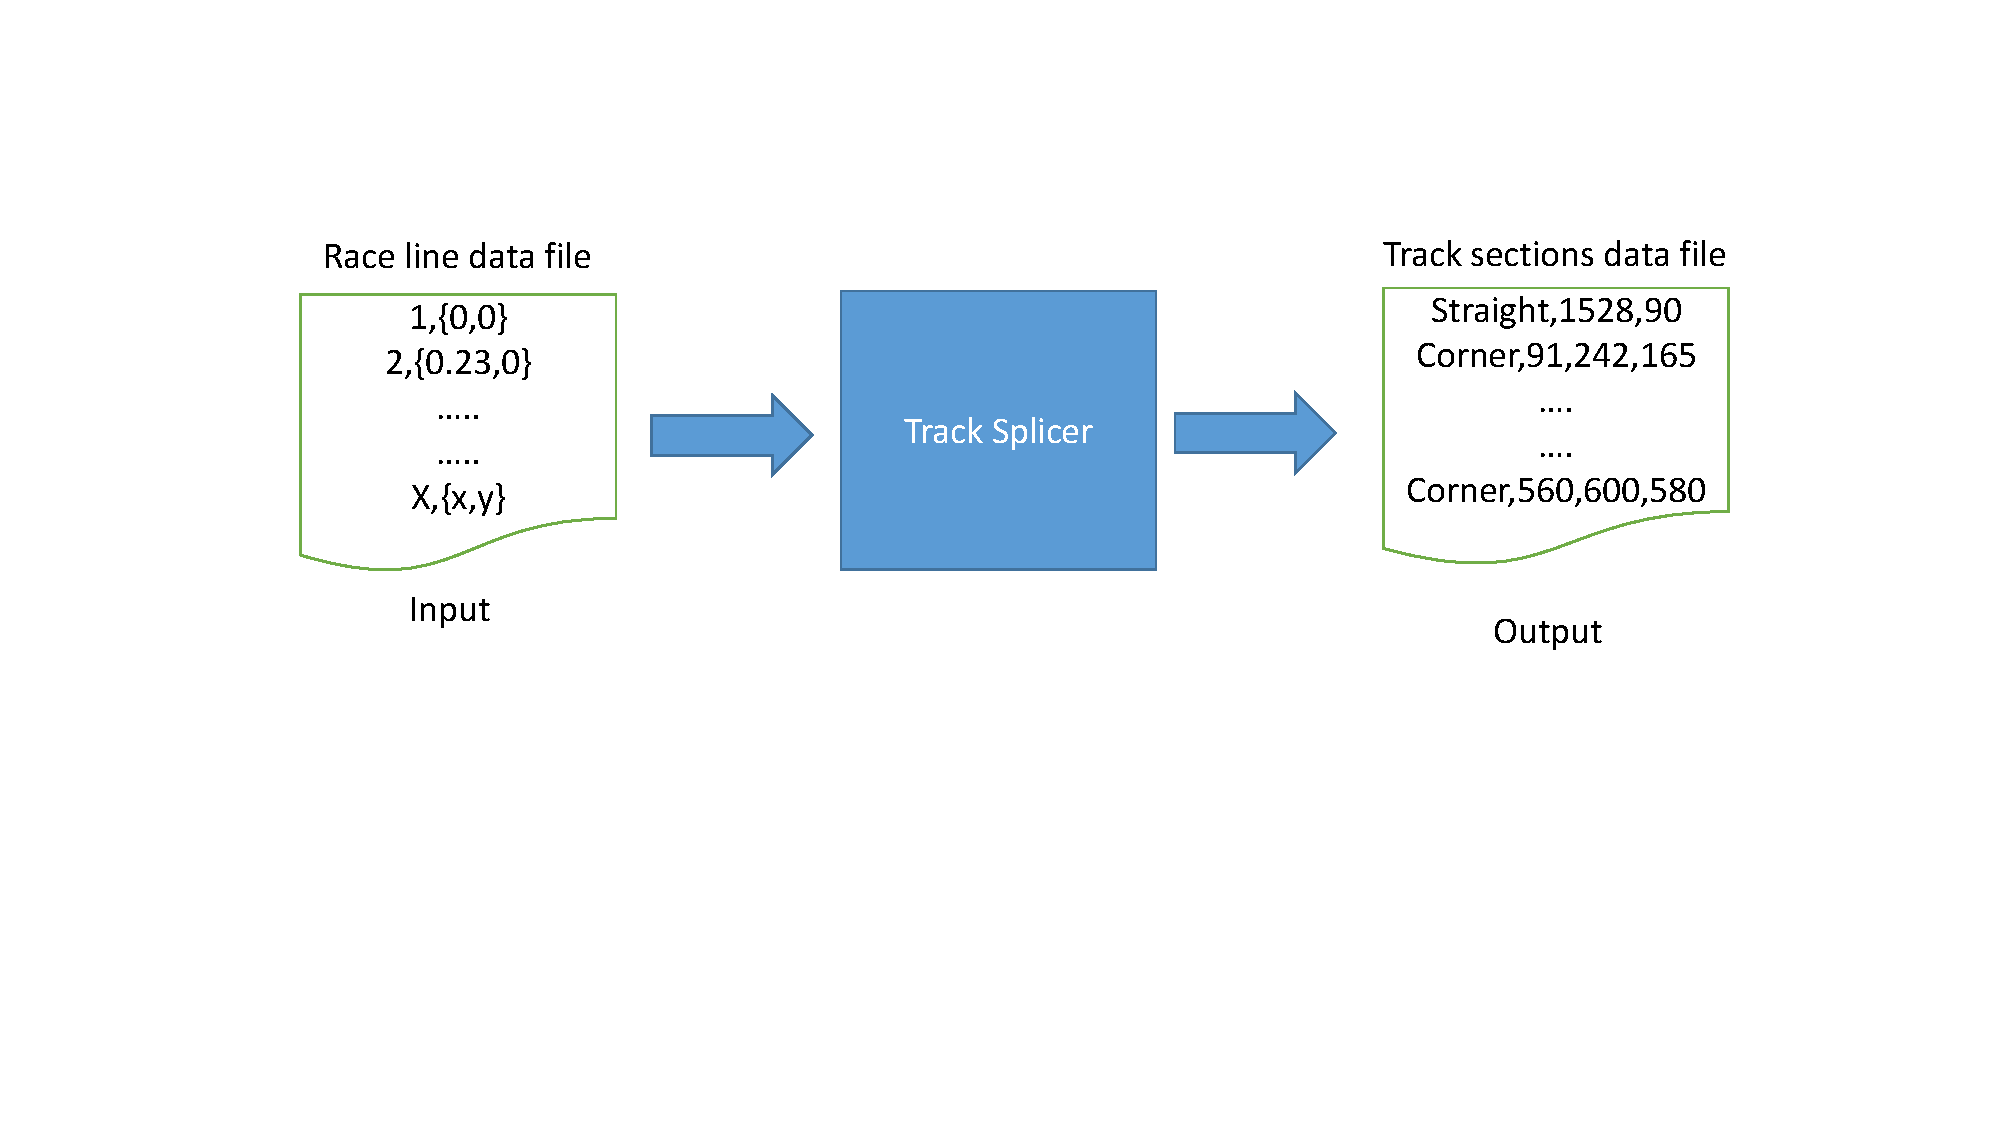
\includegraphics[width=\textwidth]{diagrams/trackspliceinputoutput.pdf}
	\caption[track splicer input out]{Track splicer input and output}
	\label{fig:diagram-trackspliceinputoutput}
\end{figure}

\begin{description}
	\item [Split the race line into straights and corners] This is done by calculating the rate of change of the line by means of vectors dot products. A cartesian coordinate p[x] as 'p1' is considered where x is the position in the array. Two other points are required p[x+1] as 'p2' and p[x+2] as 'p3'. When x is the end of the list, the first two points are used from the list. Using p1, p2 and p3, two vectors are generated, 'v1' which is a vector going from p1 to p2, and 'v2' which is a vector going from p2 to p3. The vectors are normalised as the their magnitude is irrelevant for this computation. The dot product of v1 and v2 is computed, the result is passed through the arccos function which results in the angle difference. If the angle is above a threshold value the point p1 is said to be part of a corner section, otherwise p1 is said to be part of a straight. The threshold value is customizable and is find tuned on a track by track bases.
	
	\begin{figure}[!htb]
		\centering
		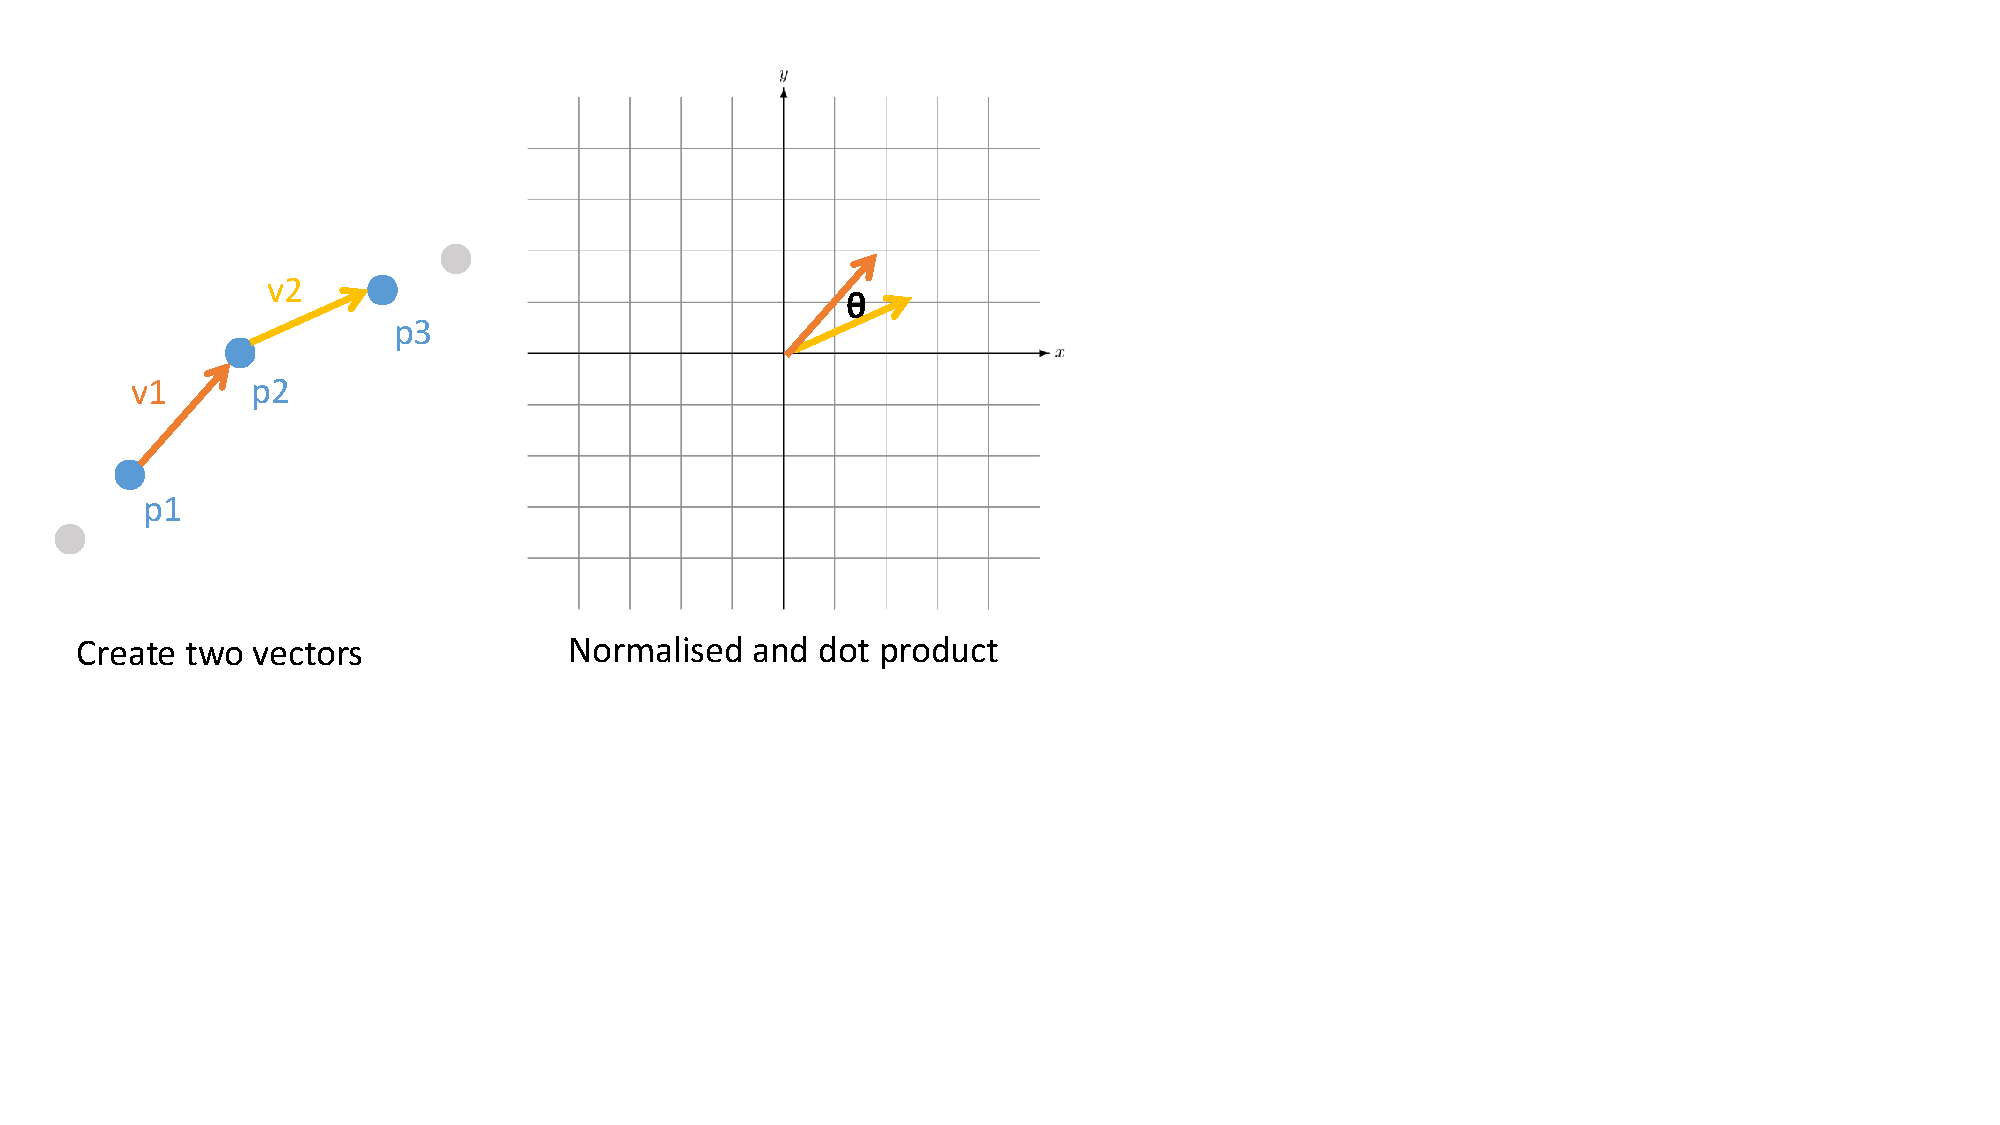
\includegraphics[width=\textwidth]{diagrams/vectorCorners.pdf}
		\caption[Splicing using vectors]{Points and vectors visualised}
		\label{fig:diagram-vectorCorners}
	\end{figure}
	
	\item [Find the mid point of a corner] The mid point of a corner is the highest point of the corner as shown in the figure. The mid point is found by going through each point. A perpendicular vector 'vP' to the first point is calculated, then a vector list vL is created containing a vector for each point as such v[x] = vector(p[x].x, p[x].y) where x is the position of the point in the array. Finally each vector in vL has the dot product with VP computed. The vector with the highest dot product result corresponds with the point which is the mid point of the corner.
	
	\begin{figure}[!htb]
		\centering
		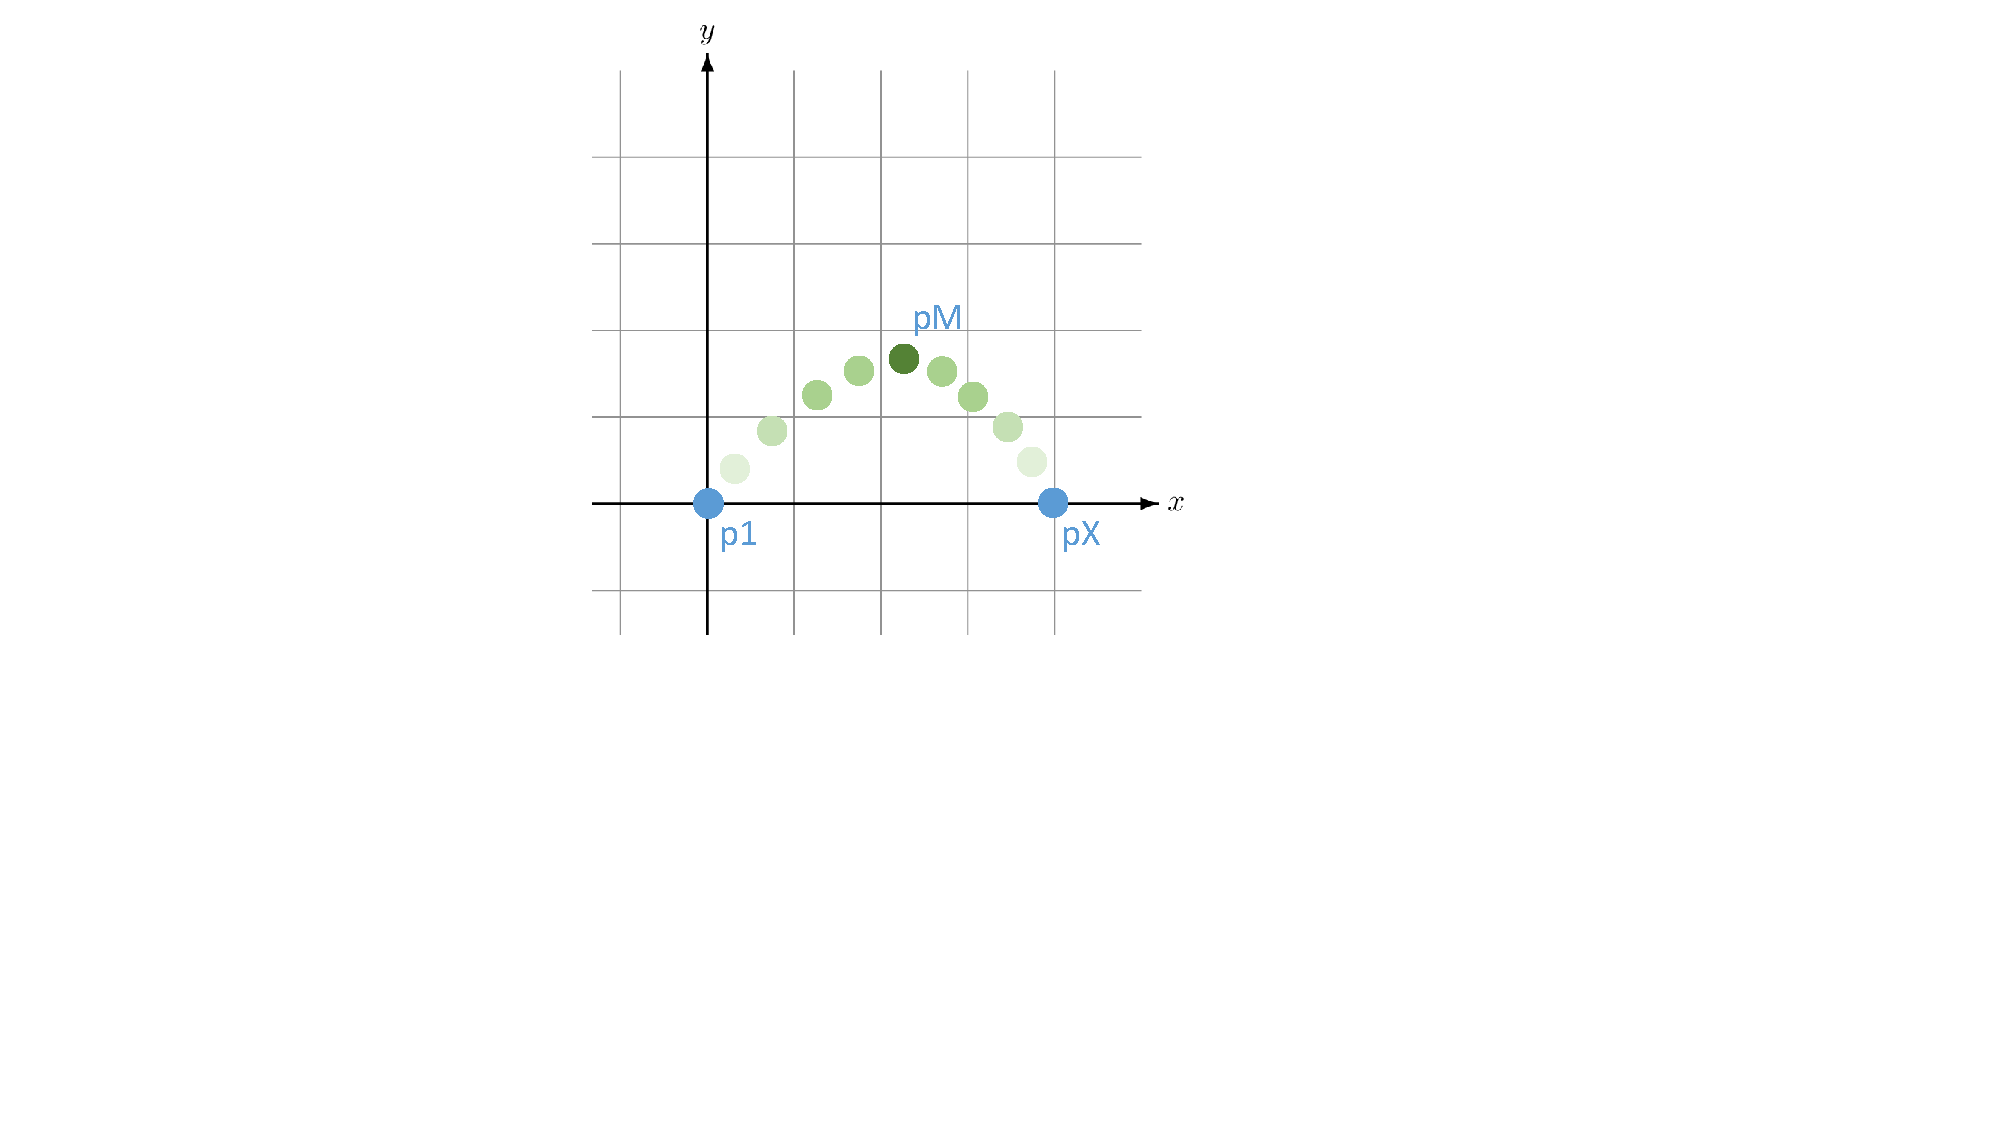
\includegraphics[height=5cm]{diagrams/cornerMidPoint.pdf}
		\caption[Corner mid point]{Finding the corner mid point}
		\textbf{p1} : First point \textbf{pM} : Corner mid point \textbf{pX} : Last point
		\label{fig:diagram-cornerMidPoint}
	\end{figure}
	
	\item [Visual representation of the race line] It was important to be able to visualise the results of the above processes in order to be able to determine the correctness of the processes. For this reasons an application with a graphic user interface was developed from which one can see the results.
	
	\begin{figure}[!htb]
		\centering
		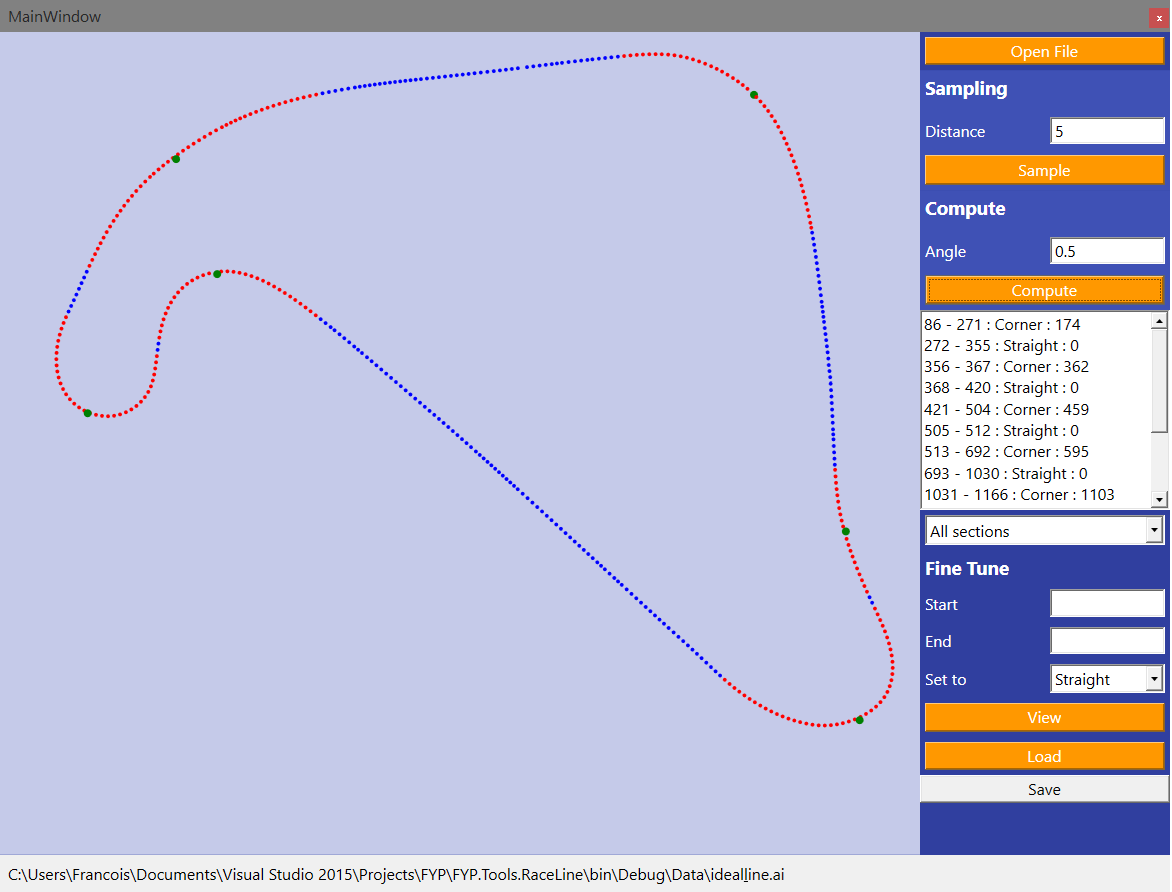
\includegraphics[height=5cm]{images/tracksplicertool}
		\caption{Track splicer tool}
		\textbf{Blue dots} : Part of a straight \textbf{Red dots} : Part of a corner \textbf{Green dots} : Corner mid point
		\label{fig:TrackSplicerTool}
	\end{figure}
	
\end{description}

\subsection{Log files Data Store}
Telemetry data log files from each sessions was inserted into a database management system by means of an extraction transfer loading processes. The process took a log file as an input and inserted the records into a table. By using a database management system it was possible to be able to store and query large amount of data in an efficient way. At first Microsoft Excel was being used however there were too many records to be stored in one sheet, further more the excel is not flexible enough to perform the same query operations which are possible with a structured query language.

\begin{figure}[!htb]
	\centering
	
\includegraphics[width=\textwidth]{diagrams/ssis.png}
	\caption{Microsoft Integration Services SQL import}
	\label{fig:ssis}
\end{figure}

\subsection{Spatial Querying}
\label{sec:imp-SpatialQuerying}
Spatial querying operations are supported by means of a quad tree data structure. Searching in a quad tree is take place in O(logn) which is a big improvement over a simple liner search which would be done in O(n). Furthermore quad tress are easily implemented and work well with two dimensional coordinates.

\begin{figure}[!htb]
	\centering
	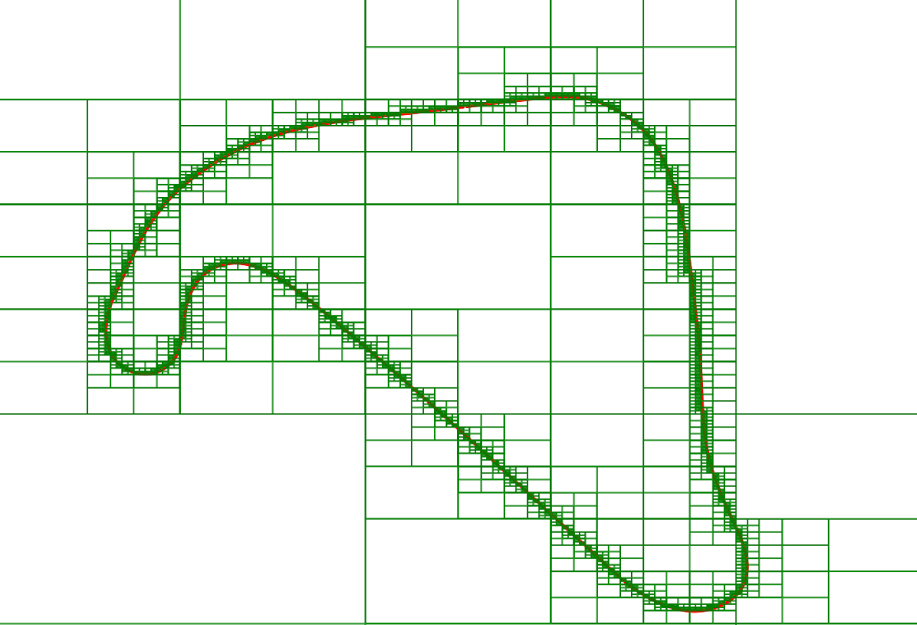
\includegraphics[height=5cm]{images/QuadTree}
	\caption{Visual representation for part of the quad tree for the Silverstone national circuit}
	\label{fig:QuadTree}
\end{figure}

\section{System Architecture}
\label{sec:imp-systemArchitecture}
The feedback system is made up of independent components which pass data to each other in order to produce the feedback instruction which is output to the user. Below is the break down of each component including an overview of their inner workings.

\begin{figure}[!htb]
	\centering
	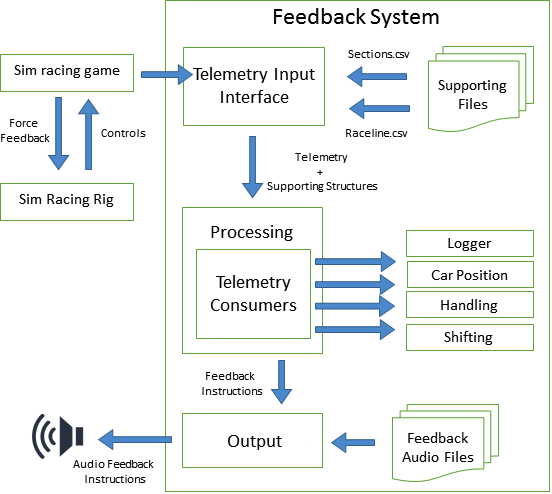
\includegraphics[height=10cm]{images/SystemArch}
	\caption{Overview of the system architecture components}
	\label{fig:SystemArch}
\end{figure}

\subsection{Telemetry Input Interface}
This components handles data inputs, two type of inputs are required, static and real time inputs. The static inputs are the ones which have been previously generated by the supporting tools. Real time input refers to the telemetry generated from the sim racing game. Assetto corsa provides a UDP server which a client can connect to, once the connection is established the game will send telemetry data.

\subsection{Processing}
Feedback processing is split into sub modules. Each module runs on a separate independent thread and gets a copy of the telemetry data passed in real time as it becomes available. Modules can be developed and plugged in without changing any other components. Having each module run on a dedicated thread ensures the system can scale horizontally making uses of all the available cores without hindering the feedback systems responsiveness. The processing component acts as a coordinator by passing data to sub modules, and listening to any feedback notification raised which are forwarded to the output interface.

\begin{figure}[!htb]
	\centering
	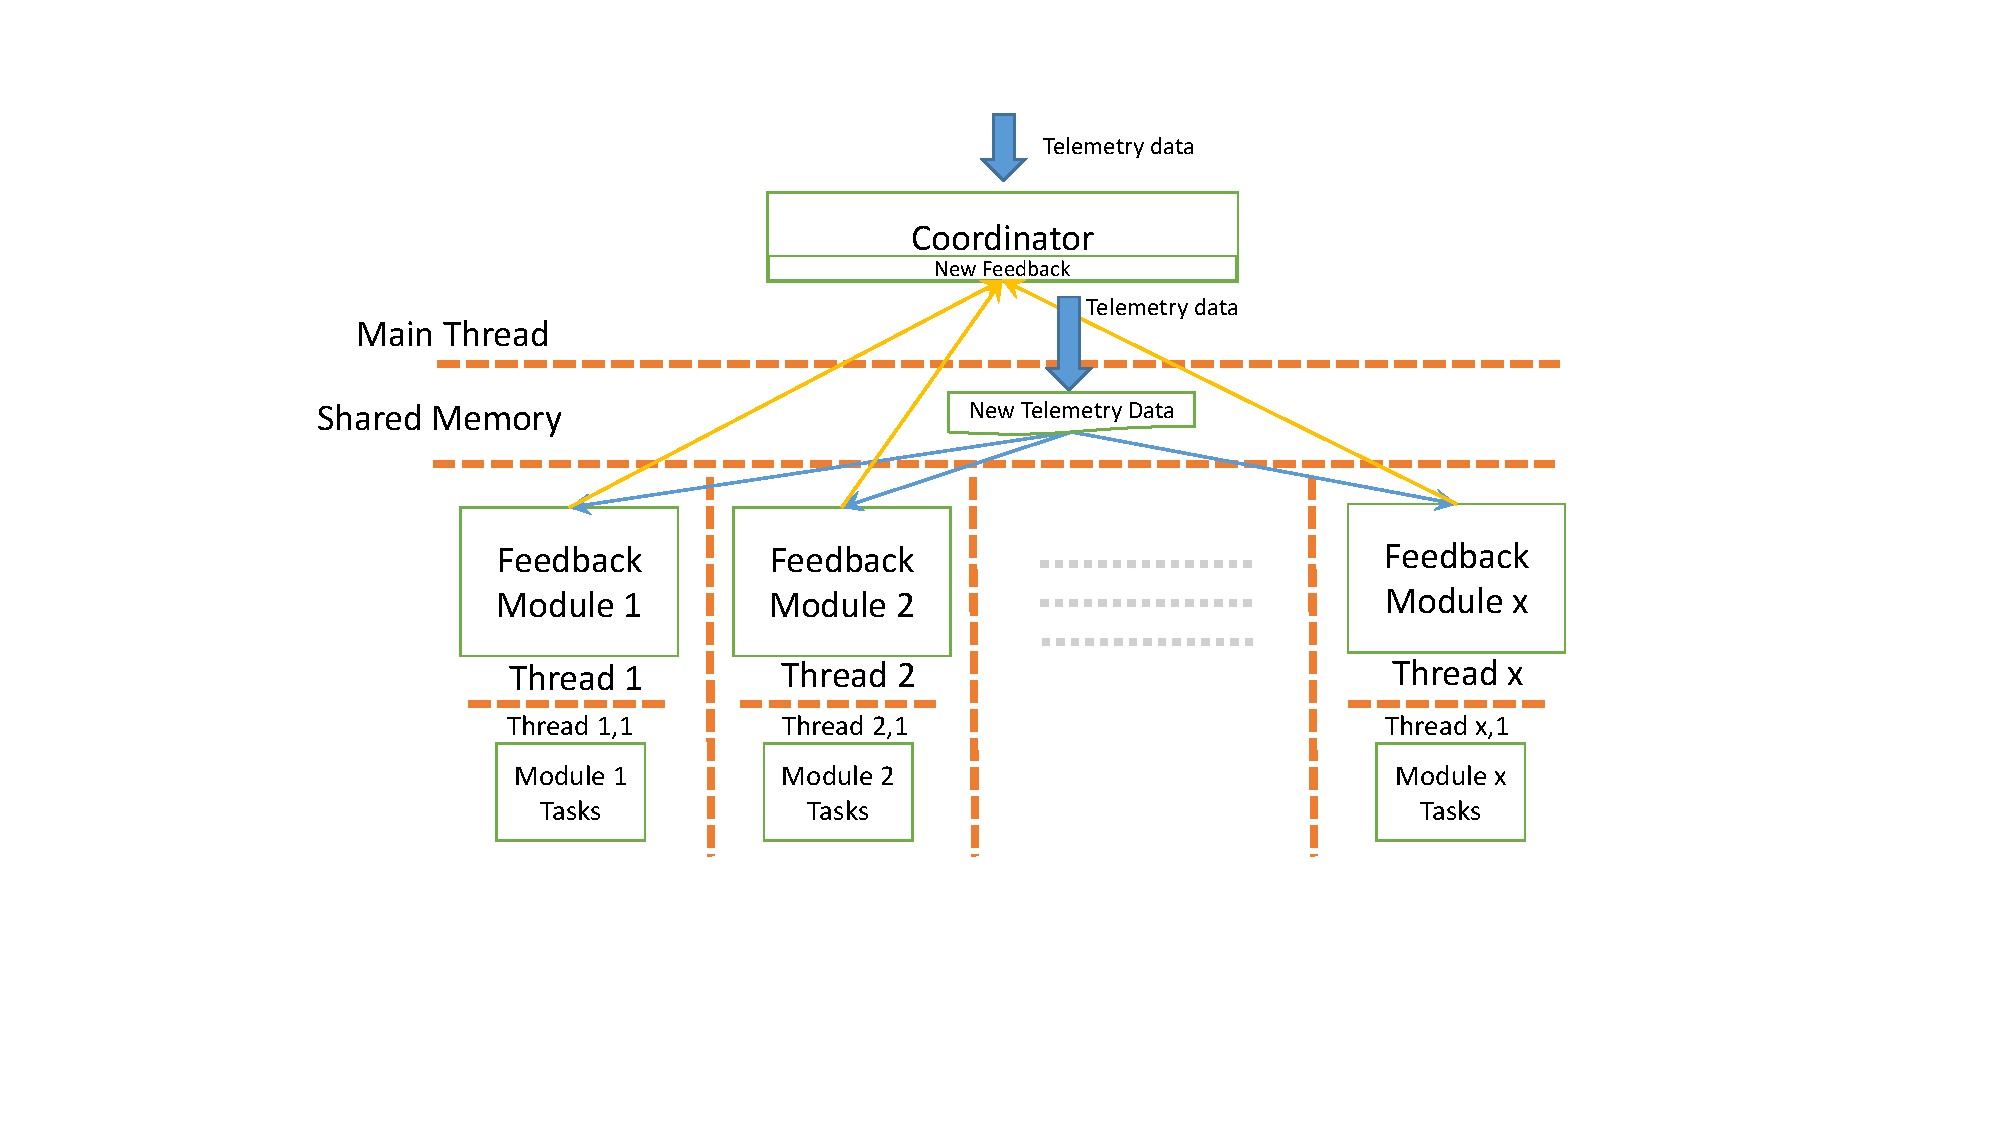
\includegraphics[width=\textwidth]{diagrams/multithreading.pdf}
	%[height=7cm]{diagrams/multithreading.pdf}
	\caption{Overview of the coordination threading}
	\label{fig:multithreading}
\end{figure}

Optimisation is also carried out within this component. This is achieved by filtering out by an expert system the feedback before being propagated to the output module. The knowledge base of the expert system is a hand crafted static one, based of rules and facts derived from the Background chapter. The inference engine works in a tiered skill based manner. At first only instructions from the basic tier are given. After the user manages to improve the basic tier skills, feedback instructions for the next tier are allowed pass to the output. In addition each module has a tolerance associated to each feedback notification it can provide. This allows the expert system to adjust how strict a module should be in raising a notification and be able to gradually make the system stricter as the user improves.

\subsection{Feedbacks being provided}
In this sub section an overview of all implemented feedback modules is given.

\textbf{Handling} component monitors for braking and acceleration behaviours. It is able to raise the following feedback notifications, 
\begin{itemize}
	\item Braking too hard
	\item Braking too light
	\item Braking in corner
	\item Losing traction to the drive wheels by applying too much power
\end{itemize}

\textbf{Car Position} component monitors for any issues which might cause the user to not adhere to the race line. As such this module can raise the following notifications 
\begin{itemize}
	\item Incorrect race line during corner
	\item Being too aggressive during a corner
	\item Not slow during a corner
	\item Track section report
\end{itemize}

\textbf{Shifting} component monitors how the user is changing gears, which allows it to raise the following notifications
\begin{itemize}
	\item Changing gear to soon
	\item Changing gear to late
	\item Taking too long to transition from one gear to another
\end{itemize}

\subsection{Output Interface}
Each possible feedback instruction which can be generated by the processing module has a static audio file associated to it. The audio files are generated from a free on line text to speech tool. The purpose of this component is to listen for feedback instruction generated by the processing component and play the corresponding audio file.